\documentclass[conference]{IEEEtran}
\IEEEoverridecommandlockouts
\usepackage{cite}
\usepackage{balance}
\usepackage{amsmath,amssymb,amsfonts}
\usepackage{graphicx}
\usepackage{textcomp}
\usepackage{xcolor}
\usepackage{booktabs}
\usepackage{tikz}
\usetikzlibrary{positioning,arrows.meta,fit,calc}
\usepackage[hidelinks]{hyperref}
\newcommand{\NTrainGauges}{193}
\newcommand{\NTestGauges}{48}
\newcommand{\NGauges}{242}
\newcommand{\AblMinutes}{3.4}
\newcommand{\NTrainRows}{1,641,197}
\newcommand{\NValRows}{349,645}
\newcommand{\NTestRows}{52,994}
\newcommand{\PosRate}{5.5}
\newcommand{\NFeat}{50}
\newcommand{\Thr}{0.45}
\newcommand{\GroupFlow}{11}
\newcommand{\GroupRain}{10}
\newcommand{\GroupWeather}{5}
\newcommand{\GroupSoil}{6}
\newcommand{\GroupSeason}{2}
\newcommand{\GroupStatic}{16}
\newcommand{\XgbBA}{0.898}
\newcommand{\XgbPR}{0.737}
\newcommand{\XgbRec}{0.902}
\newcommand{\XgbPrec}{0.328}
\newcommand{\XgbBALo}{0.886}
\newcommand{\XgbBAHi}{0.910}
\newcommand{\PersBA}{0.750}
\newcommand{\PersPR}{0.428}
\newcommand{\PersRec}{0.508}
\newcommand{\PersPrec}{0.789}
\newcommand{\PersBALo}{0.724}
\newcommand{\PersBAHi}{0.778}
\newcommand{\ClimBA}{0.802}
\newcommand{\ClimPR}{0.203}
\newcommand{\ClimRec}{0.891}
\newcommand{\ClimPrec}{0.152}
\newcommand{\ClimBALo}{0.774}
\newcommand{\ClimBAHi}{0.829}
\newcommand{\LstmBA}{0.873}
\newcommand{\LstmPR}{0.589}
\newcommand{\LstmRec}{0.826}
\newcommand{\LstmPrec}{0.376}
\newcommand{\LstmBALo}{0.829}
\newcommand{\LstmBAHi}{0.911}
\newcommand{\NoFlowBA}{0.853}
\newcommand{\NoFlowPR}{0.494}
\newcommand{\NoFlowRec}{0.865}
\newcommand{\NoFlowPrec}{0.239}
\newcommand{\NoFlowBALo}{0.820}
\newcommand{\NoFlowBAHi}{0.880}
\newcommand{\DiffPersLo}{0.123}
\newcommand{\DiffPersHi}{0.175}
\newcommand{\LstmCov}{100}
\newcommand{\LstmCompare}{On the rows it covers, the model (0.898) and the simulation (0.873) were statistically indistinguishable in balanced accuracy, although only the model is a real forecast.}
\newcommand{\AblAllBA}{0.898}
\newcommand{\AblAllPR}{0.736}
\newcommand{\AlarmsThr}{150.2}
\newcommand{\PrecSeventyFive}{0.539}
\newcommand{\RecSeventyFive}{0.760}
\newcommand{\EceRaw}{0.102}
\newcommand{\EceIso}{0.005}
\newcommand{\CalWord}{over-confident}
\newcommand{\PgN}{46}
\newcommand{\PgMed}{0.900}
\newcommand{\PgQOne}{0.860}
\newcommand{\PgQThree}{0.926}
\newcommand{\PgMin}{0.769}
\newcommand{\EvN}{266}
\newcommand{\EvXgbWarn}{91.4}
\newcommand{\EvLstmWarn}{83.5}
\newcommand{\EvClimWarn}{89.5}
\newcommand{\EvPersWarn}{0.0}
\newcommand{\EvNoFlowWarn}{94.0}
\newcommand{\LeakRandBA}{0.915}
\newcommand{\LeakRandPR}{0.810}
\newcommand{\LeakTimeBA}{0.892}
\newcommand{\LeakTimePR}{0.724}
\newcommand{\LeakSpaceBA}{0.905}
\newcommand{\LeakSpacePR}{0.789}
\newcommand{\LeakSpTiBA}{0.898}
\newcommand{\LeakSpTiPR}{0.736}
\newcommand{\LeakGapBA}{1.7}
\newcommand{\LeakGapPR}{7.4}
\newcommand{\LeakText}{The random row split gave the highest balanced accuracy, 0.915, against 0.898 on unseen gauges in later years, and the two bootstrap intervals do not overlap. Random splitting inflated balanced accuracy by 1.7 points and PR-AUC by 7.4 points. PR-AUC ranged from 0.724 (new years) to 0.810 (random rows). Holding out later years lowered PR-AUC more than holding out gauges (0.724 against 0.789), so a temporal split matters at least as much as a spatial one. In the spatial protocol, the test years are also the years from which each gauge's flood threshold was computed.}
\newcommand{\LeakDiscuss}{the evaluation protocol alone moved balanced accuracy by 1.7 points (Table~\ref{tab:leak}), so scores from random row splits overstate what a forecaster will achieve at a new gauge, and published Indian flood models can only be compared under the same split.}
\newcommand{\LeakConclude}{A random row split would have reported a balanced accuracy 1.7 points higher.}
\newcommand{\LeakAbstract}{Scoring the same model on random rows raised balanced accuracy to 0.915, an inflation of 1.7 points.}
\newcommand{\LeadOne}{96.7}
\newcommand{\LeadOneRise}{90.3}
\newcommand{\LeadTwo}{93.3}
\newcommand{\LeadTwoRise}{85.2}
\newcommand{\LeadThree}{89.5}
\newcommand{\LeadThreeRise}{80.0}
\newcommand{\FpMonsoonPct}{86}
\newcommand{\MonPrec}{0.311}
\newcommand{\OthPrec}{0.415}
\newcommand{\MonAlarms}{372}
\newcommand{\OthAlarms}{36}
\newcommand{\NearMissMon}{21}
\newcommand{\FaRatioMon}{41}
\newcommand{\PgGauges}{46}
\newcommand{\RhoArea}{0.44}
\newcommand{\PArea}{0.002}
\newcommand{\PMinOther}{0.64}
\newcommand{\WarnThreeXgb}{63.9}
\newcommand{\WarnThreeLstm}{78.9}
\newcommand{\WarnThreeClim}{89.1}
\newcommand{\EvGauges}{44}
\newcommand{\MeanLeadXgb}{2.58}
\newcommand{\ImpFlow}{67.5}
\newcommand{\ImpRain}{13.6}
\newcommand{\ImpWeather}{7.3}
\newcommand{\ImpTopOne}{40.5}
\newcommand{\ImpTopTwo}{23.9}
\newcommand{\ImpRainDay}{8.5}
\newcommand{\RelHiConf}{0.97}
\newcommand{\RelHiFreq}{0.75}
\newcommand{\OnsetAll}{0.852}
\newcommand{\OnsetNoFlow}{0.846}
\newcommand{\OnsetFlowOnly}{0.810}


\begin{document}

\title{Forecasting Three-Day Flood Exceedance at Gauges\\
Unseen in Space and Time: A Leakage-Controlled\\
Benchmark on CAMELS-IND}

%<AUTHORS>
\author{
\IEEEauthorblockN{Nandhakumar T}
\IEEEauthorblockA{\textit{Department of Information Technology}\\
\textit{Sona College of Technology}\\
Salem, Tamil Nadu, India\\
nandhakumartm93@gmail.com}
\and
\IEEEauthorblockN{Balakarthikeyan B S}
\IEEEauthorblockA{\textit{Department of Artificial Intelligence and Data Science}\\
\textit{Sona College of Technology}\\
Salem, Tamil Nadu, India\\
balasan2626@gmail.com}
\and
\IEEEauthorblockN{Gowthaman J}
\IEEEauthorblockA{\textit{Department of Artificial Intelligence and Data Science}\\
\textit{Sona College of Technology}\\
Salem, Tamil Nadu, India\\
gowthamanjanadhran@gmail.com}
\and
\IEEEauthorblockN{Abhishek S}
\IEEEauthorblockA{\textit{Department of Artificial Intelligence and Data Science}\\
\textit{Sona College of Technology}\\
Salem, Tamil Nadu, India\\
abisheksengodan18@gmail.com}
}
%</AUTHORS>

\maketitle

\begin{abstract}
Flood warnings in India are issued gauge by gauge, yet machine-learning flood forecasters are often scored on random row splits that let neighbouring days of the same river leak between training and test data. We build a leakage-controlled benchmark on CAMELS-IND for one operational question: will a gauge's flow reach its flood level within the next three days? We train on \NTrainGauges{} gauges for 1980--2008, select models and thresholds on 2009--2014, and test once on \NTestGauges{} unseen gauges in 2015--2020. A gradient-boosted model reached a balanced accuracy of \XgbBA{} (95\% gauge-bootstrap interval \XgbBALo--\XgbBAHi) and a PR-AUC of \XgbPR, against \PersBA{} and \PersPR{} for persistence, \ClimBA{} and \ClimPR{} for gauge climatology, and \LstmBA{} and \LstmPR{} for the dataset's regional LSTM simulation, which is driven by the observed future rain. \LeakAbstract{} Removing all streamflow inputs lowered balanced accuracy to \NoFlowBA. Recall fell from \LeadOne\% one day ahead to \LeadThree\% three days ahead, skill rose with catchment area, and \FpMonsoonPct\% of false alarms came in the monsoon, typically on rivers that peaked well below their flood level. With a precision of \XgbPrec, a positive forecast should trigger review by an officer.
\end{abstract}

\begin{IEEEkeywords}
flood forecasting, CAMELS-IND, data leakage, gradient boosting, hydrological benchmark
\end{IEEEkeywords}

\section{Introduction}
An emergency officer watching an Indian river gauge needs a plain answer: is the flow likely to reach its flood level in the next few days? Machine-learning models trained on many catchments now simulate streamflow well, even in basins without a gauge record \cite{Kratzert2019a,Kratzert2019b,Nearing2024}. Reported skill, however, depends on how a model is evaluated. When rows are split at random, days from the same flood fall on both sides of the split, and part of the test score then rewards memory of the event \cite{Kapoor2023,Roberts2017}.

India now has a large-sample dataset to study this properly. CAMELS-IND provides daily forcing, observed streamflow and catchment attributes for peninsular Indian catchments \cite{Mangukiya2025}, in the format of the CAMELS family \cite{Newman2015,Addor2017}. It also ships a regional LSTM simulation of streamflow, which gives a strong deep-learning reference at no extra cost. What is missing is a short-range flood-exceedance benchmark on these gauges that controls leakage, compares against simple and strong references, and reports the numbers an operations room needs: alarm rates, onset lead time and calibration.

We build such a benchmark. Our contributions are:
\begin{enumerate}
\item A leakage-controlled task and split: gauges held out in space and time, flood thresholds from training years only, model and threshold selection on validation only, and a single use of the test set (Fig.~\ref{fig:split}).
\item A measurement of how much the evaluation protocol changes the score: one model configuration scored under random, temporal, spatial and space-and-time splits.
\item A comparison with persistence, the gauge's own climatology and the CAMELS-IND regional LSTM simulation, with gauge-cluster bootstrap intervals.
\item A feature-group ablation that shows what the forecast relies on, including a variant that needs no streamflow reading at forecast time.
\item An operational analysis of operating points, calibration, per-gauge skill and the lead time of warnings before flood onsets.
\end{enumerate}

\section{Related Work}
\textit{Large-sample learning.} The CAMELS datasets standardised forcing, flow and attributes across hundreds of basins \cite{Newman2015,Addor2017}. LSTMs trained on them learn regional behaviour \cite{Kratzert2019a}, predict ungauged basins \cite{Kratzert2019b} and simulate extremes better than conceptual models \cite{Frame2022}; at global scale, a learned model forecasts extreme floods in ungauged watersheds with skill comparable to an operational system \cite{Nearing2024}. Graph models that encode the river network have so far not beaten models that ignore it \cite{Kirschstein2024}. Most of this work simulates streamflow; flood \emph{exceedance}, the quantity a warning is issued on, is usually derived afterwards.

\textit{Operational forecasting.} Physically based ensemble systems such as GloFAS \cite{Alfieri2013} dominate operational flood forecasting \cite{Cloke2009}. Machine learning has also reached operations: a system run for India and Bangladesh combines learned river-stage forecasts with inundation models \cite{Nevo2022}. In India, the INDOFLOODS catalogue documents historical events \cite{Kuntla2025} and many studies apply tree ensembles or neural networks to single basins \cite{Mosavi2018}, often with random splits.

\textit{Evaluation.} Leakage through the split is a leading cause of irreproducible machine-learning results \cite{Kapoor2023}, and data with spatial or temporal structure need blocked validation \cite{Roberts2017}. For rare events, precision--recall curves are more informative than ROC curves \cite{Saito2015}, and probabilistic forecasts should be checked for calibration \cite{Brier1950}.

Table~\ref{tab:pos} places our work. To our knowledge, no study has benchmarked short-range flood-exceedance forecasting on CAMELS-IND with a space-and-time held-out split against both a learned streamflow simulation and simple references.

\begin{table}[t]
\caption{Position of this study among related work}
\label{tab:pos}
\centering
\footnotesize
\setlength{\tabcolsep}{2.2pt}
\begin{tabular}{lllll}
\toprule
Study & Region & Target & Held out & References\\
\midrule
\cite{Kratzert2019b} & USA & daily flow & basins & conceptual models\\
\cite{Nearing2024} & global & flood events & basins & GloFAS\\
\cite{Kirschstein2024} & Europe & flow & time & LSTM\\
\cite{Mangukiya2025} & India & daily flow & -- & regional LSTM\\
This work & India & 3-day exceedance & gauges + time & LSTM, clim., pers.\\
\bottomrule
\multicolumn{5}{l}{\scriptsize clim. = gauge climatology; pers. = persistence; -- = dataset paper.}\\
\end{tabular}
\end{table}

\section{Data and Task}
\subsection{Target}
For gauge $g$ on day $t$ the target is
\begin{equation}
y_{g,t}=\mathbb{1}\Big[\max_{h\in\{1,2,3\}} Q_{g,t+h}\ \ge\ q^{95}_g\Big],
\label{eq:target}
\end{equation}
where $Q$ is observed streamflow and $q^{95}_g$ is the 95th percentile of the gauge's flow over the training years 1980--2008 only. A three-day horizon matches the time an officer needs to stage teams. Days without a flow observation in the horizon are dropped.

\subsection{Inputs}
Table~\ref{tab:feat} lists the \NFeat{} inputs, all known at the end of day $t$. Flow features are scaled by $q^{95}_g$, so they read as ``how close the river is to its flood level''. Hydrological signatures of CAMELS-IND are excluded, because they are computed over the full 1980--2020 record and would leak test-period information; future rainfall is excluded as well.

\begin{table}[t]
\caption{Input groups (all known at the end of day $t$)}
\label{tab:feat}
\centering
\footnotesize
\setlength{\tabcolsep}{3pt}
\begin{tabular}{llc}
\toprule
Group & Content & Inputs\\
\midrule
Streamflow & lags 0--3, changes, 7/30-day means and maxima & \GroupFlow\\
Rainfall & lags 0--3, 3--90-day sums, 7-day maximum & \GroupRain\\
Weather & temperature, humidity, evapotranspiration & \GroupWeather\\
Soil moisture & four layers and recent changes & \GroupSoil\\
Season & day of year (sine, cosine) & \GroupSeason\\
Catchment & area, slope, aridity, land cover, soils & \GroupStatic\\
\bottomrule
\end{tabular}
\end{table}

\subsection{Split}
Fig.~\ref{fig:split} shows the split. The observed-streamflow file lists \NGauges{} gauges, and all of them have forcing data and at least three years of flow in 1980--2008, which our pipeline requires; the dataset authors' stricter availability filter keeps 228 \cite{Mangukiya2025}.A group split puts 20\% of gauges aside (seed 42), so the primary test asks about rivers the model has never seen, in years it has never seen. Training uses the other gauges in 1980--2008 (\NTrainRows{} gauge-days), validation the same gauges in 2009--2014 (\NValRows), and the test the unseen gauges in 2015--2020, all labelled by (\ref{eq:target}) (\NTestRows{} gauge-days, of which \PosRate\% are flood windows).

\begin{figure}[t]
\centering
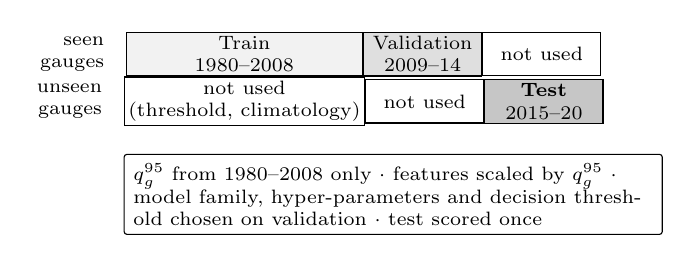
\begin{tikzpicture}[font=\scriptsize,
  cell/.style={draw, minimum height=0.55cm, align=center, inner sep=1.5pt},
  arr/.style={-{Latex[length=1.4mm]}, semithick}]
\node[cell, minimum width=3.0cm, fill=gray!10] (tr) at (0,0) {Train\\1980--2008};
\node[cell, minimum width=1.5cm, fill=gray!25, right=0pt of tr] (va) {Validation\\2009--14};
\node[cell, minimum width=1.5cm, right=0pt of va] (sx) {not used};
\node[cell, minimum width=3.0cm, below=0pt of tr] (ux) {not used\\(threshold, climatology)};
\node[cell, minimum width=1.5cm, right=0pt of ux] (uy) {not used};
\node[cell, minimum width=1.5cm, fill=gray!45, right=0pt of uy] (te) {\textbf{Test}\\2015--20};
\node[left=0.15cm of tr, align=right] {seen\\gauges};
\node[left=0.15cm of ux, align=right] {unseen\\gauges};
\node[draw, rounded corners=1pt, align=left, below=0.35cm of ux.south west, anchor=north west, text width=6.6cm] (rules)
 {$q^{95}_g$ from 1980--2008 only $\cdot$ features scaled by $q^{95}_g$ $\cdot$ model family, hyper-parameters and decision threshold chosen on validation $\cdot$ test scored once};
\end{tikzpicture}
\caption{Leakage-controlled split. The primary test uses gauges and years that played no part in training, model selection or threshold choice. The unseen gauges' 1980--2008 record is used only to set their flood threshold and climatology.}
\label{fig:split}
\end{figure}

\section{Methods}
\textit{Model.} Seven candidates (logistic regression, random forest, histogram gradient boosting and four XGBoost \cite{Chen2016} configurations) were compared on validation balanced accuracy, and the decision threshold of the selected depth-6 XGBoost model, \Thr, was set on validation as well. With $\mathrm{TPR}$ and $\mathrm{TNR}$ the true positive and true negative rates,
\begin{equation}
\mathrm{BA}=\tfrac12\left(\mathrm{TPR}+\mathrm{TNR}\right).
\label{eq:ba}
\end{equation}

\textit{References.} \emph{Persistence} forecasts a flood window if the river is above its flood level today. \emph{Climatology} forecasts the gauge's own 1980--2008 rate of flood windows within $\pm15$ days of the calendar day. The \emph{LSTM simulation} is the regional LSTM streamflow of CAMELS-IND \cite{Mangukiya2025}, scored as $\max_{h\le3}\hat Q_{g,t+h}/q^{95}_g$. It is driven by observed forcing, so it sees the rain of days $t{+}1$ to $t{+}3$, which no real forecast has; it is therefore an optimistic reference rather than a competitor. Thresholds of the references were set on validation like the model's.

\textit{Analyses.} We refit the selected configuration on the same 500,000-row training sample with one input group removed at a time, and with the streamflow and season inputs only. Gain importance is read from the selected model itself. Confidence intervals come from 1,000 resamples of the test gauges, which keeps each river's days together. Calibration is the expected calibration error over ten bins, before and after isotonic regression fitted on validation. A flood onset is a day on which the river reaches $q^{95}_g$ after at least seven days below it; a method warns of it if it forecasts a flood window one, two or three days earlier. For lead-day and seasonal analyses, a flood day at lead $h$ is a day $t$ with $Q_{g,t+h}\ge q^{95}_g$, and the monsoon is June to September.

\textit{Reproducibility.} Every split and resample uses seed 42, and the 49 test gauges are stored with the model metadata. Re-scoring the stored model reproduces its recorded test balanced accuracy exactly, and every number in this paper is generated from the experiment outputs by a script that also checks each claim made about it. Fitting one ablation model took a median of \AblMinutes{} minutes on a laptop CPU with four threads.

\section{Results}
\subsection{Skill on Unseen Gauges}
Table~\ref{tab:main} and Fig.~\ref{fig:pr} give the main comparison, with balanced accuracy as defined in (\ref{eq:ba}). The model was clearly better than persistence and climatology in balanced accuracy, recall and PR-AUC, and its bootstrap interval for the gain in balanced accuracy over persistence (\DiffPersLo--\DiffPersHi) excludes zero. Persistence was more precise (\PersPrec{} against \XgbPrec): when the river is already high it is usually right, but it misses every flood that has not yet begun. The model's recall of \XgbRec{} means that it found nine in ten flood windows at rivers it had never seen.

\begin{table}[t]
\caption{Three-day exceedance on \NTestGauges{} unseen gauges, 2015--2020}
\label{tab:main}
\centering
\footnotesize
\setlength{\tabcolsep}{1.6pt}
\begin{tabular}{lcccccc}
\toprule
Method & BA & 95\% CI & PR-AUC & Rec. & Prec. & F1\\
\midrule
XGBoost (ours) & 0.898 & 0.886--0.910 & 0.737 & 0.902 & 0.328 & 0.481\\
No-flow XGB. & 0.853 & 0.820--0.880 & 0.494 & 0.865 & 0.239 & 0.374\\
LSTM sim.$^\dagger$ & 0.873 & 0.829--0.911 & 0.589 & 0.826 & 0.376 & 0.517\\
Climatology & 0.802 & 0.774--0.829 & 0.203 & 0.891 & 0.152 & 0.260\\
Persistence & 0.750 & 0.724--0.778 & 0.428 & 0.508 & 0.789 & 0.618\\
\bottomrule
\multicolumn{7}{l}{\scriptsize CI: gauge-cluster bootstrap.}\\
\multicolumn{7}{l}{\scriptsize $^\dagger$Driven by observed future rain; scored on its \LstmCov\% of rows.}\\
\end{tabular}
\end{table}

\begin{figure}[t]
\centering
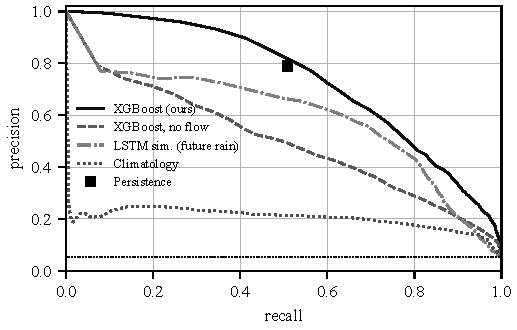
\includegraphics[width=\columnwidth]{fig_pr.pdf}
\caption{Precision--recall curves on the unseen test gauges. The square is persistence; the dotted line is the flood rate.}
\label{fig:pr}
\end{figure}

The LSTM simulation is a demanding reference because it knows the rain that is still to fall. \LstmCompare{} The model reaches its skill from today's information alone, largely because it reads how close the river already is to its flood level.

\subsection{Effect of the Evaluation Protocol}
To measure what the split itself does to the score, we trained the same configuration on a 500,000-row sample under four protocols, each with its own validation set for early stopping and threshold, and scored it once (Table~\ref{tab:leak}). \LeakText{}

\begin{table}[t]
\caption{Same model, four evaluation protocols}
\label{tab:leak}
\centering
\footnotesize
\setlength{\tabcolsep}{2.4pt}
\begin{tabular}{lccccc}
\toprule
Test set & Gauges & BA & 95\% CI & PR-AUC & Prec.\\
\midrule
Random rows & 242 & 0.915 & 0.911--0.919 & 0.810 & 0.426\\
New years & 181 & 0.892 & 0.885--0.898 & 0.724 & 0.349\\
New gauges & 49 & 0.905 & 0.898--0.912 & 0.789 & 0.424\\
New gauges and years & 48 & 0.898 & 0.886--0.911 & 0.736 & 0.340\\
\bottomrule
\multicolumn{6}{l}{\scriptsize Random: 70/10/20\% of all gauge-days.}\\
\multicolumn{6}{l}{\scriptsize Others trained on seen gauges, 1980--2008. New years:}\\
\multicolumn{6}{l}{\scriptsize seen gauges, 2015--20; new gauges: unseen, 1980--2008.}\\
\end{tabular}
\end{table}

\subsection{What the Forecast Relies On}
Table~\ref{tab:abl} shows the ablation. Over all rows, removing the streamflow inputs cost the most, lowering balanced accuracy from \AblAllBA{} to \NoFlowBA{} and PR-AUC from \AblAllPR{} to \NoFlowPR, while removing soil moisture, rainfall or catchment attributes cost little. Much of that score, however, comes from rivers that are already high and stay high. On onset rows, where the river is still below its flood level and a warning matters most, the picture reverses: without streamflow the onset balanced accuracy fell only from \OnsetAll{} to \OnsetNoFlow, whereas streamflow and season alone reached \OnsetFlowOnly. Today's flow tells whether a flood will continue; rain, soil moisture and weather tell whether one will start. The no-flow variant also beat climatology overall (\NoFlowBA{} against \ClimBA), so it is a usable fallback when a gauge reading is missing.

The selected model's own gain importance (Fig.~\ref{fig:imp}) agrees with the overall picture: streamflow inputs account for \ImpFlow\% of the total gain, led by today's flow relative to the flood level (\ImpTopOne\%) and its seven-day maximum (\ImpTopTwo\%), followed by rainfall (\ImpRain\%, of which today's rain alone \ImpRainDay\%). Gain importance is known to favour inputs used in many splits, which is why we base the conclusions above on the ablation and use the importance only as a check.

\begin{figure}[t]
\centering
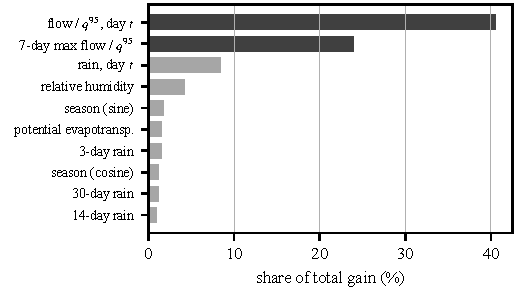
\includegraphics[width=\columnwidth]{fig_imp.pdf}
\caption{Ten largest shares of total gain in the selected model. Dark bars are streamflow inputs.}
\label{fig:imp}
\end{figure}

\begin{table}[t]
\caption{Feature-group ablation (same 500k training sample)}
\label{tab:abl}
\centering
\footnotesize
\setlength{\tabcolsep}{3pt}
\begin{tabular}{lccccc}
\toprule
Inputs & $n$ & BA & PR-AUC & Rec. & Onset BA\\
\midrule
All inputs & 50 & 0.898 & 0.736 & 0.897 & 0.852\\
No streamflow & 39 & 0.853 & 0.494 & 0.865 & 0.846\\
No catchment & 34 & 0.895 & 0.734 & 0.907 & 0.855\\
No soil moisture & 44 & 0.896 & 0.732 & 0.895 & 0.854\\
No rainfall & 40 & 0.897 & 0.730 & 0.901 & 0.857\\
Streamflow + season & 13 & 0.875 & 0.685 & 0.882 & 0.810\\
\bottomrule
\multicolumn{6}{l}{\scriptsize Onset BA: rows where the river is below its flood level on day $t$.}\\
\end{tabular}
\end{table}

\subsection{Operational Behaviour}
Precision is the main weakness. At the validation threshold the model raised \AlarmsThr{} alarms per 1,000 gauge-days at a precision of \XgbPrec{} (Table~\ref{tab:ops}); raising the threshold to 0.75 halved the alarms and lifted precision to \PrecSeventyFive, at a recall of \RecSeventyFive. Because a positive forecast in our system leads to human review rather than automatic action, the validation threshold is a reasonable default. The raw probabilities were \CalWord{} (ECE \EceRaw); isotonic recalibration on validation data lowered the ECE to \EceIso{}. Fig.~\ref{fig:rel} shows the size of the problem: in the highest well-populated bin the raw forecast averaged \RelHiConf{} while floods followed in \RelHiFreq{} of cases. This is consistent with the positive-class weighting used in training, which shifts scores upward. The alarms at the validation threshold are computed from the raw score and are unaffected, but a raw score must not be shown to an officer as a probability; the recalibrated one can be.

\begin{figure}[t]
\centering
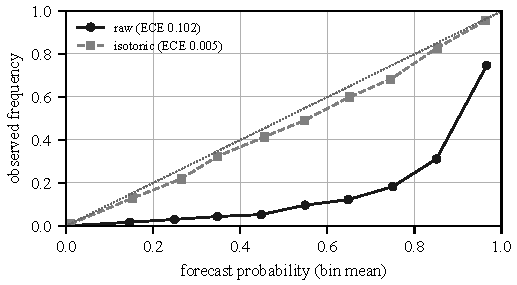
\includegraphics[width=\columnwidth]{fig_rel.pdf}
\caption{Reliability of the forecast probabilities on the unseen test gauges, before and after isotonic recalibration fitted on validation data (bins with at least 50 gauge-days).}
\label{fig:rel}
\end{figure}

\begin{table}[t]
\caption{Operating points on the test set (threshold \Thr{} set on validation)}
\label{tab:ops}
\centering
\footnotesize
\begin{tabular}{cccc}
\toprule
Threshold & Recall & Precision & Alarms / 1000 days\\
\midrule
0.30 & 0.942 & 0.261 & 197.2\\
0.45 & 0.902 & 0.328 & 150.2\\
0.60 & 0.845 & 0.413 & 111.6\\
0.75 & 0.760 & 0.539 & 77.0\\
\bottomrule
\end{tabular}
\end{table}


Table~\ref{tab:warn} gives the lead of the warnings. The model warned three days ahead for \WarnThreeXgb\% of the \EvN{} onsets at \EvGauges{} gauges, with a mean lead of \MeanLeadXgb{} days when it warned. Climatology (\WarnThreeClim\%) and the LSTM simulation (\WarnThreeLstm\%) appear better on this measure, but for different reasons: climatology raises an alarm on most monsoon days, which its precision of \ClimPrec{} reflects, and the LSTM simulation is given the rain that is still to fall. Lead counts alone therefore reward methods that alarm constantly, and they should be read together with precision.

\begin{table}[t]
\caption{Warning lead before the \EvN{} flood onsets (\% of onsets)}
\label{tab:warn}
\centering
\footnotesize
\setlength{\tabcolsep}{3pt}
\begin{tabular}{lccccc}
\toprule
Method & 3 days & 2 days & 1 day & none & Mean lead\\
\midrule
XGBoost (ours) & 63.9 & 16.5 & 10.9 & 8.6 & 2.58\\
No-flow XGB. & 72.2 & 14.7 & 7.1 & 6.0 & 2.69\\
LSTM sim.$^\dagger$ & 78.9 & 4.5 & 0.0 & 16.5 & 2.95\\
Climatology & 89.1 & 0.4 & 0.0 & 10.5 & 3.00\\
\bottomrule
\multicolumn{6}{l}{\scriptsize Mean lead in days, over warned onsets. $^\dagger$Driven by observed future rain.}\\
\end{tabular}
\end{table}

Skill was consistent across rivers: over the \PgN{} test gauges with at least one flood window, the median per-gauge balanced accuracy was \PgMed{} (interquartile range \PgQOne--\PgQThree), and the worst gauge reached \PgMin. For the \EvN{} flood onsets at the test gauges, the model warned one to three days ahead in \EvXgbWarn\% of cases, against \EvLstmWarn\% for the LSTM simulation, \EvClimWarn\% for climatology and \EvPersWarn\% for persistence, which by definition cannot anticipate an onset. The no-flow variant warned of \EvNoFlowWarn\%, more than the full model, in line with the ablation: an onset is announced by the weather more than by the river.

\subsection{Where the Forecast Succeeds and Fails}
\textit{Lead day.} The target pools three lead days, so Table~\ref{tab:lead} splits the recall by the day on which the river is above its flood level. The model raised an alarm on day $t$ for \LeadOne\% of flood days at $t{+}1$, \LeadTwo\% at $t{+}2$ and \LeadThree\% at $t{+}3$. On rivers still below their flood level on day $t$, which is where a warning is useful, the rates were lower: \LeadOneRise\%, \LeadTwoRise\% and \LeadThreeRise\%.

\begin{table}[t]
\caption{Recall by lead day on the unseen test gauges}
\label{tab:lead}
\centering
\footnotesize
\begin{tabular}{ccccc}
\toprule
Lead & \multicolumn{2}{c}{All flood days} & \multicolumn{2}{c}{River below $q^{95}_g$ on day $t$}\\
$h$ (days) & $n$ & Recall \% & $n$ & Recall \%\\
\midrule
1 & 1875 & 96.7 & 474 & 90.3\\
2 & 1874 & 93.3 & 681 & 85.2\\
3 & 1874 & 89.5 & 830 & 80.0\\
\bottomrule
\end{tabular}
\end{table}

\textit{Season.} Table~\ref{tab:season} separates the monsoon months. In June to September the model raised \MonAlarms{} alarms per 1,000 gauge-days at a precision of \MonPrec, against \OthAlarms{} and \OthPrec{} in the rest of the year, and \FpMonsoonPct\% of all false alarms fell in the monsoon. Most of these were not near misses: in the median monsoon false alarm the river peaked at \FaRatioMon\% of its flood level over the next three days, and only \NearMissMon\% of them reached 70--100\%. The model thus responds to monsoon conditions in general more than to an approaching flood.

\begin{table}[t]
\caption{Skill by season on the unseen test gauges}
\label{tab:season}
\centering
\footnotesize
\setlength{\tabcolsep}{2.6pt}
\begin{tabular}{lcccccc}
\toprule
Months & Gauge-days & Flood \% & BA & Rec. & Prec. & Alarms/1000\\
\midrule
Jun--Sep & 17,992 & 12.7 & 0.811 & 0.915 & 0.311 & 372\\
Oct--May & 35,002 & 1.8 & 0.918 & 0.857 & 0.415 & 36\\
\bottomrule
\end{tabular}
\end{table}

\textit{Catchment.} Fig.~\ref{fig:area} plots the per-gauge balanced accuracy of the \PgGauges{} test gauges with flood windows against catchment area. Skill rose with area (Spearman $\rho=\RhoArea$, $p=\PArea$), which is consistent with large rivers rising slowly enough for today's flow to describe the next three days. Aridity, mean rainfall and slope showed no relation ($p\ge\PMinOther$). Small, fast catchments are where rainfall forecasts are likely to help most.

\begin{figure}[t]
\centering
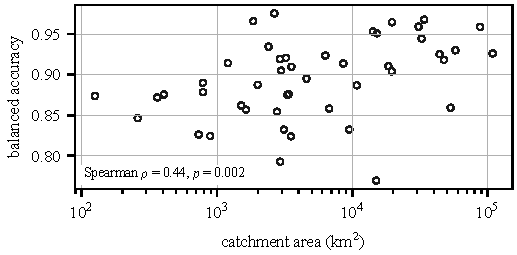
\includegraphics[width=\columnwidth]{fig_area.pdf}
\caption{Per-gauge balanced accuracy against catchment area on the unseen test gauges (log scale).}
\label{fig:area}
\end{figure}

\section{Discussion and Limitations}
Three findings matter for practice. First, the inputs play different roles. Today's flow carries the overall score, but the start of a flood is predicted from rain, soil moisture and weather, so an operations room needs both a reliable gauge feed and good meteorological inputs; when the feed fails, the no-flow variant is a better fallback than climatology. Second, precision is the weak point, and it is mainly a monsoon problem: most false alarms fell in June to September on rivers that stayed well below their flood level. The LSTM simulation, which is given the observed future rain, reached a precision of only \LstmPrec, so better rainfall information alone may not fix it. Until it is fixed, a positive forecast should start a review by an officer, and an evacuation needs further evidence. Third, \LeakDiscuss{}


Fig.~\ref{fig:deploy} turns these findings into a deployment design. The forecast runs on the full input set while the gauge feed is live and falls back to the no-flow model when it is not; its score is recalibrated before an officer sees it, and an alarm opens a review instead of an order.

\begin{figure}[t]
\centering
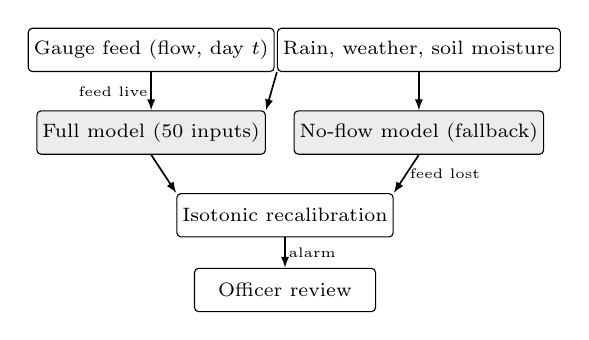
\begin{tikzpicture}[font=\scriptsize,
  box/.style={draw, rounded corners=1.5pt, align=center, minimum height=0.55cm, minimum width=2.3cm, inner sep=2pt},
  arr/.style={-{Latex[length=1.4mm]}, semithick}, lab/.style={font=\tiny, inner sep=1pt}]
\node[box] (g) at (0,0) {Gauge feed (flow, day $t$)};
\node[box] (w) at (3.4,0) {Rain, weather, soil moisture};
\node[box, fill=gray!15] (f) at (0,-1.05) {Full model (\NFeat{} inputs)};
\node[box, fill=gray!15] (n) at (3.4,-1.05) {No-flow model (fallback)};
\node[box] (c) at (1.7,-2.1) {Isotonic recalibration};
\node[box] (o) at (1.7,-3.05) {Officer review};
\draw[arr] (g) -- node[lab, left]{feed live} (f);
\draw[arr] (w) -- (n);
\draw[arr] (w.south west) -- (f.north east);
\draw[arr] (f.south) -- (c.north west);
\draw[arr] (n.south) -- node[lab, right]{feed lost} (c.north east);
\draw[arr] (c) -- node[lab, right]{alarm} (o);
\end{tikzpicture}
\caption{Deployment suggested by the results: the full model while the gauge feed is live, the no-flow model when it fails, recalibrated scores, and human review of every alarm.}
\label{fig:deploy}
\end{figure}

For studies that report flood forecasts on Indian rivers, the results suggest a minimal protocol:
\begin{enumerate}
\item hold out both gauges and later years, and report the split with the score (Table~\ref{tab:leak});
\item set flood thresholds, models and decision thresholds from training and validation years only;
\item report precision and alarm rates beside balanced accuracy, by season (Table~\ref{tab:season});
\item report skill on onset rows, where the river is still below its flood level (Table~\ref{tab:abl});
\item check calibration before showing a score as a probability (Fig.~\ref{fig:rel}).
\end{enumerate}

The study has limits. The CAMELS-IND gauges are in peninsular India, so skill may not transfer to Himalayan or Brahmaputra rivers. The 95th-percentile threshold is a statistical proxy for an official danger level. The LSTM reference was trained by the dataset authors on a design we do not control, and because it sees future rain the comparison with it is indicative only. We pool three lead days into one target and use one fixed random group split; a basin-aware split, which holds out whole river basins, may be stricter still. The ablation and protocol models were refitted on a 500,000-row sample, so they are compared with each other; the all-input refit scored \AblAllBA, as the selected model trained on all rows did (\XgbBA).

\section{Conclusion}
On CAMELS-IND gauges held out in space and time, a gradient-boosted model forecast three-day flood exceedance with a balanced accuracy of \XgbBA{} and a PR-AUC of \XgbPR, well above persistence and the gauge's own climatology, and warned of \EvXgbWarn\% of flood onsets in advance. Its overall score rests mostly on the current river state, while flood onsets depend on meteorological inputs. Its skill is lower at later lead days and in smaller catchments, and its precision of \XgbPrec{}, lowest in the monsoon, makes it a trigger for review by an officer. \LeakConclude{} The split and the protocol give a reference against which other forecasters on Indian rivers can be compared.

\section*{Acknowledgment}
The authors thank the CAMELS-IND and INDOFLOODS dataset authors for openly available data.
In line with the IEEE policy on AI-generated content, the authors disclose that Claude (Anthropic) was used to help edit and restructure the text of all sections and to draft the experiment and plotting scripts. All experiments use the authors' own software and fixed seeds. The authors checked every number, claim and reference and take full responsibility for the content.

\balance
\begin{thebibliography}{00}
\bibitem{Kratzert2019a} F. Kratzert, D. Klotz, G. Shalev, G. Klambauer, S. Hochreiter, and G. Nearing, ``Towards learning universal, regional, and local hydrological behaviors via machine learning applied to large-sample datasets,'' \textit{Hydrol. Earth Syst. Sci.}, vol. 23, pp. 5089--5110, 2019, doi: 10.5194/hess-23-5089-2019.
\bibitem{Kratzert2019b} F. Kratzert, D. Klotz, M. Herrnegger, A. K. Sampson, S. Hochreiter, and G. S. Nearing, ``Toward improved predictions in ungauged basins: Exploiting the power of machine learning,'' \textit{Water Resour. Res.}, vol. 55, pp. 11344--11354, 2019, doi: 10.1029/2019WR026065.
\bibitem{Nearing2024} G. Nearing \textit{et al.}, ``Global prediction of extreme floods in ungauged watersheds,'' \textit{Nature}, vol. 627, pp. 559--563, 2024, doi: 10.1038/s41586-024-07145-1.
\bibitem{Kapoor2023} S. Kapoor and A. Narayanan, ``Leakage and the reproducibility crisis in machine-learning-based science,'' \textit{Patterns}, vol. 4, no. 9, Art. no. 100804, 2023, doi: 10.1016/j.patter.2023.100804.
\bibitem{Roberts2017} D. R. Roberts \textit{et al.}, ``Cross-validation strategies for data with temporal, spatial, hierarchical, or phylogenetic structure,'' \textit{Ecography}, vol. 40, no. 8, pp. 913--929, 2017, doi: 10.1111/ecog.02881.
\bibitem{Mangukiya2025} N. K. Mangukiya \textit{et al.}, ``CAMELS-IND: Hydrometeorological time series and catchment attributes for 228 catchments in Peninsular India,'' \textit{Earth Syst. Sci. Data}, vol. 17, pp. 461--491, 2025, doi: 10.5194/essd-17-461-2025.
\bibitem{Newman2015} A. J. Newman \textit{et al.}, ``Development of a large-sample watershed-scale hydrometeorological data set for the contiguous USA: Data set characteristics and assessment of regional variability in hydrologic model performance,'' \textit{Hydrol. Earth Syst. Sci.}, vol. 19, pp. 209--223, 2015, doi: 10.5194/hess-19-209-2015.
\bibitem{Addor2017} N. Addor, A. J. Newman, N. Mizukami, and M. P. Clark, ``The CAMELS data set: Catchment attributes and meteorology for large-sample studies,'' \textit{Hydrol. Earth Syst. Sci.}, vol. 21, pp. 5293--5313, 2017, doi: 10.5194/hess-21-5293-2017.
\bibitem{Frame2022} J. M. Frame \textit{et al.}, ``Deep learning rainfall--runoff predictions of extreme events,'' \textit{Hydrol. Earth Syst. Sci.}, vol. 26, pp. 3377--3392, 2022, doi: 10.5194/hess-26-3377-2022.
\bibitem{Kirschstein2024} N. Kirschstein and Y. Sun, ``The merit of river network topology for neural flood forecasting,'' in \textit{Proc. 41st Int. Conf. Mach. Learn. (ICML)}, PMLR vol. 235, Vienna, Austria, 2024, pp. 24713--24725.
\bibitem{Alfieri2013} L. Alfieri \textit{et al.}, ``GloFAS -- global ensemble streamflow forecasting and flood early warning,'' \textit{Hydrol. Earth Syst. Sci.}, vol. 17, pp. 1161--1175, 2013, doi: 10.5194/hess-17-1161-2013.
\bibitem{Cloke2009} H. L. Cloke and F. Pappenberger, ``Ensemble flood forecasting: A review,'' \textit{J. Hydrol.}, vol. 375, pp. 613--626, 2009, doi: 10.1016/j.jhydrol.2009.06.005.
\bibitem{Nevo2022} S. Nevo \textit{et al.}, ``Flood forecasting with machine learning models in an operational framework,'' \textit{Hydrol. Earth Syst. Sci.}, vol. 26, no. 15, pp. 4013--4032, 2022, doi: 10.5194/hess-26-4013-2022.
\bibitem{Kuntla2025} S. K. Kuntla and M. Saharia, ``INDOFLOODS: A comprehensive database for flood events in India enhanced with catchment attributes,'' \textit{Bull. Amer. Meteorol. Soc.}, vol. 106, no. 2, pp. E333--E343, 2025, doi: 10.1175/BAMS-D-24-0008.1.
\bibitem{Mosavi2018} A. Mosavi, P. Ozturk, and K.-W. Chau, ``Flood prediction using machine learning models: Literature review,'' \textit{Water}, vol. 10, no. 11, Art. no. 1536, 2018, doi: 10.3390/w10111536.
\bibitem{Saito2015} T. Saito and M. Rehmsmeier, ``The precision-recall plot is more informative than the ROC plot when evaluating binary classifiers on imbalanced datasets,'' \textit{PLoS ONE}, vol. 10, no. 3, Art. no. e0118432, 2015, doi: 10.1371/journal.pone.0118432.
\bibitem{Brier1950} G. W. Brier, ``Verification of forecasts expressed in terms of probability,'' \textit{Mon. Weather Rev.}, vol. 78, no. 1, pp. 1--3, 1950.
\bibitem{Chen2016} T. Chen and C. Guestrin, ``XGBoost: A scalable tree boosting system,'' in \textit{Proc. 22nd ACM SIGKDD Int. Conf. Knowl. Discov. Data Min.}, 2016, pp. 785--794, doi: 10.1145/2939672.2939785.
\end{thebibliography}

\end{document}
